% !TEX TS-program = pdflatex
% !TEX encoding = UTF-8 Unicode

% This is a simple template for a LaTeX document using the "article" class.
% See "book", "report", "letter" for other types of document.

\documentclass[11pt, titlepage]{article} % use larger type; default would be 10pt

\usepackage[utf8]{inputenc} % set input encoding (not needed with XeLaTeX)

\usepackage{lipsum}

%%% Some CONSTANTS
\newcommand{\kDocTitle}{TicText Project Documentation}
\newcommand{\kDocVersion}{1}

%%% Examples of Article customizations
% These packages are optional, depending whether you want the features they provide.
% See the LaTeX Companion or other references for full information.

%%% PAGE DIMENSIONS
\usepackage{geometry} % to change the page dimensions
\geometry{letterpaper} % or letterpaper (US) or a5paper or....
% \geometry{margin=2in} % for example, change the margins to 2 inches all round
% \geometry{landscape} % set up the page for landscape
%   read geometry.pdf for detailed page layout information

\usepackage{graphicx} % support the \includegraphics command and options
\graphicspath{ {images/}{images/uml/} }

% \usepackage[parfill]{parskip} % Activate to begin paragraphs with an empty line rather than an indent

%%% PACKAGES
\usepackage{booktabs} % for much better looking tables
\usepackage{array} % for better arrays (eg matrices) in maths
\usepackage{paralist} % very flexible & customisable lists (eg. enumerate/itemize, etc.)
\usepackage{verbatim} % adds environment for commenting out blocks of text & for better verbatim
\usepackage{subfig} % make it possible to include more than one captioned figure/table in a single float
% These packages are all incorporated in the memoir class to one degree or another...

%%% HEADERS & FOOTERS
\usepackage{fancyhdr} % This should be set AFTER setting up the page geometry
\pagestyle{fancy} % options: empty , plain , fancy
\renewcommand{\headrulewidth}{1pt} % customise the layout...
\lhead{\kDocTitle}
\chead{}
\rhead{Version \kDocVersion}
\lfoot{}
\cfoot{\thepage}
\rfoot{}

%%% SECTION TITLE APPEARANCE
\usepackage{sectsty}
\allsectionsfont{\sffamily\mdseries\upshape} % (See the fntguide.pdf for font help)
% (This matches ConTeXt defaults)

%%% ToC (table of contents) APPEARANCE
\usepackage[nottoc,notlof,notlot]{tocbibind} % Put the bibliography in the ToC
\usepackage[titles,subfigure]{tocloft} % Alter the style of the Table of Contents
\renewcommand{\cftsecfont}{\rmfamily\mdseries\upshape}
\renewcommand{\cftsecpagefont}{\rmfamily\mdseries\upshape} % No bold!

\usepackage{dialogue}
\usepackage[table]{xcolor}
\usepackage{float}
\usepackage{attrib}
\usepackage{hyperref}
%%% END Article customizations

%%% The "real" document content comes below...

\title{

\includegraphics[width=8cm]{icon}\\
\kDocTitle\\
\large{Version \kDocVersion}
}
\author{
	Terrence Katzenbaer, Kevin Chen, Chengkan Huang, Jack Arendt, Georgy Petukhov
	\footnote{Ordered by primary writer, then repository contributors sorted by descending number of commits.}
}
\date{May 3, 2015} % Activate to display a given date or no date (if empty),
         % otherwise the current date is printed 

\begin{document}
\maketitle
\tableofcontents

\clearpage
% Welcome
\section{Welcome}
Hello, reader and possible new employee at the prestiguous TicText organization. This document exists to help familiarize you with this project and its history. We will first introduce what TicText is, our motiviation, and even the biggest risks/challenges we face. Then, you will learn the software development processes we follow. Next, you will read a brief overview of the project's requirements and specifications before diving into the current architecture and design. Finally, we hope a brief outline of future plans will help you find what you want to work on.

\begin{flushright}
Let's get started, Tic Tok!
\end{flushright}

\subsection{Prerequisites}
\begin{itemize}
	\item Xcode 6, preferably the latest version
	\item iOS 7
\end{itemize}

\subsection{Setting up your Xcode project}
\begin{enumerate}
	\item After downloading the latest copy of the repository, install all project dependencies from CocoaPods by running,
		\begin{verbatim}
		cd TicText-iOS
		pod install
		\end{verbatim}
	\item Open the Xcode workspace at \verb|TicText-iOS/TicText.xcworkspace|.
	\item Set up a, or ask permissions to our development, TicText app on Parse.
	\item Copy the environment's application id and client key into \verb|AppDelegate.m|:
		\begin{verbatim}
		[Parse setApplicationId:@"APPLICATION_ID" clientKey:@"CLIENT_KEY"];
		\end{verbatim}
	\item Finally, select the \verb|TicText| target and go to \verb|Build Phases|. Under \verb|Upload Symbol Files|, update line 3 to point to your Cloud Code folder, if any. If you're not using Cloud Code, feel free to remove the \verb|Upload Symbol Files| section.
\end{enumerate}

\subsection{Configuring TicText's Facebook integration}
\begin{enumerate}
	\item Set up a, or ask permission to our development, Facebook app at \url{http://developers.facebook.com/apps}.
	\item Set up a URL scheme for \verb|fbFACEBOOK_APP_ID|, where \verb|FACEBOOK_APP_ID| is your Facebook app's id.
	\item Add your Facebook app id to \verb|Info.plist| in the \verb|FacebookAppID| key.
\end{enumerate}

\subsection{Cloud Code}
Add your Parse app id and master key to \verb|TicText-iOS/CloudCode/config/global.json|, then type \verb|parse deploy| from the command line at \verb|TicText-cloud|. See the \href{https://parse.com/docs/cloud_code_guide#clt}{Cloud Code Guide} for more information about the \verb|parse| CLI.

% Welcome
\section{Getting Started}
\subsection{Prerequisites}
\begin{itemize}
	\item Xcode 6, preferably the latest version
	\item iOS 7
\end{itemize}

\subsection{Setting up your Xcode project}
\begin{enumerate}
	\item After downloading the latest copy of the repository, install all project dependencies from CocoaPods by running,
		\begin{verbatim}
		cd TicText-iOS
		pod install
		\end{verbatim}
	\item Open the Xcode workspace at \verb|TicText-iOS/TicText.xcworkspace|.
	\item Set up a, or ask permissions to our development, TicText app on Parse.
	\item Copy the environment's application id and client key into \verb|AppDelegate.m|:
		\begin{verbatim}
		[Parse setApplicationId:@"APPLICATION_ID" clientKey:@"CLIENT_KEY"];
		\end{verbatim}
	\item Finally, select the \verb|TicText| target and go to \verb|Build Phases|. Under \verb|Upload Symbol Files|, update line 3 to point to your Cloud Code folder, if any. If you're not using Cloud Code, feel free to remove the \verb|Upload Symbol Files| section.
\end{enumerate}

\subsection{Configuring TicText's Facebook integration}
\begin{enumerate}
	\item Set up a, or ask permission to our development, Facebook app at \url{http://developers.facebook.com/apps}.
	\item Set up a URL scheme for \verb|fbFACEBOOK_APP_ID|, where \verb|FACEBOOK_APP_ID| is your Facebook app's id.
	\item Add your Facebook app id to \verb|Info.plist| in the \verb|FacebookAppID| key.
\end{enumerate}

\subsection{Cloud Code}
Add your Parse app id and master key to \verb|TicText-iOS/CloudCode/config/global.json|, then type \verb|parse deploy| from the command line at \verb|TicText-cloud|. See the \href{https://parse.com/docs/cloud_code_guide#clt}{Cloud Code Guide} for more information about the \verb|parse| CLI.

% What is TicText?
\clearpage
\section{What is TicText?}
%% Brief Description
\subsection{Brief Description}
TicText is an iOS messaging app that allows you to send expire-able text with your friends. We call this kind of text "Tic", as in the sound of a clock counting down (Tic Tok, Tic Tok...). For each Tic sent to your friends, you will be able to set a time duration, which will be the amount of time before the Tic got expired and becomes unable for your friend to retrieve its content. That is to say, the recipient can only retrieve the content from our server within a certain time period after the sender sent the Tic. Here is an example of a possible scenario of using TicText:

\begin{dialogue}
	\speak{John} \direct{\refer{He} is drunk at 3am and sends a tic using \refer{His Phone} to \refer{Mary} with a 60 minute expiration time. The tic reads...}
	
		\medskip
		Hey babe, I miss you so much and I really regret breaking up with you...
	
		\medskip
		\direct{\refer{Mary} (while sleeping) receives a notification on her phone.}
	\speak{Mary's Phone} Someone has just sent you a Tic! Swipe to read before it's too late. Tic Tok...
	
		\medskip
		\direct{The next morning, \refer{Mary} saw the notification and opened the app. The only thing left was...}
	\speak{TicText on Mary's Phone} Sorry you've missed a Tic which expired on 4:00 am.
\end{dialogue}

TicText would also let you to send a Tic anonymously - even if the recipient saw the notification in time, he/she still won't be able to see the sender's name.

We believe TicText is also capable of creating romance in many ways. But in the example above, well, hopefully TicText just avoid something awkward or even more. 
%% Motivation
\subsection{Motivation}
We would like to build something brings people joy and more importantly, works even with limited amount of users. So we gave up on the ideas related to sharing, social networking, or dating, and focused on single user or 1-on-1 experiences. I believe TicText could be something we, especially the younger generation, would enjoy. Also, building a mobile app with modern technologies will always be challenging and exciting. From my past experiences, I'm sure we could learn a lot and have fun as well. 

%% Risks/Challenges
\subsection{Risks/Challenges}
One of the biggest challenges would be building a good-looking UI with great user experience. There wouldn't be many features in TicText so UX will be the top priority with no doubts. In the meantime, we have to think about the security of all the Tics as well. The last thing we want is compromising user's privacy. In order to do that, we need more than beautiful code, but also coding in the "right way" using the "right tools".


% Formal Software Development Process
\clearpage
\section{Formal Software Development Process}
The process followed by your team (make use of your essay if you are taking CS429) - (5 points)

Make sure to address the issues of iterative development, refactoring, testing and collaborative development (even if you are not using XP, you have to address these issues in your documentation).
\\

In the software development world, every project ultimately descends into chaos. Teams proactively battle against this entropy using formal software development methods. These methods can slow a projects descent, but they can, when used effectively, stall the descent entirely. One method that we learned and applied last semester in Software Engineering was Extreme Programming. Extreme Programming is a branch under Agile Software Development methodology and derives many of its practices from Agile Software Development including fast iteration cycles, use cases, and user stories; but, Extreme Programming differs from a typical Agile Software Development methodology through pair programming and complete unit testing. 

While my group last semester followed many of the practices of Extreme Programming, we did not adhere as strictly to pair programming. Why did the students in my group not desire pair programming, especially when I received multiple second-person accounts of groups that flawlessly utilized pair programming? Could group dynamic, individual skill, an unnecessary byproduct of our interspersed and erratic location on campus at any given time, or something else determine pair programming’s necessity and success? I believe that all of the aforementioned concerns contribute in peer hesitation to adopt and consistently practice pair programming. Some group atmospheres do not support or encourage their members to admit unfamiliarity or inexperience. Other individuals feel their skill does not necessitate someone else watching over their shoulder as they crank out clean code–line by line. And the sheer size and scatterness of the campus make it difficult for students to easily coordinate a place and time for pair programming. Because of the reality of resistance to pair programming, my group this semester has adopted it on an as-needed basis. We hope that this compromise will let skilled individuals maintain their efficiency while also helping the bottom line–those that may not be experts in the technology.

To improve team efficiency and facilitate grading, the instructors frequently require students to use Subversion: a program (more accurately “a lifestyle choice”) that helps software developers maintain and track all changes to, or version, a code repository–similar to what I’m doing manually for this essay. My group this semester hopes to improve efficiency adjustments to our project’s software development method by versioning our code with Git instead of Subversion. The biggest difference between Git and Subversion is how collaboration is organized. Subversion uses centralized remote repositories, which means that each collaborator syncs every change with a single master repository over the Internet. Git, on the other hand, uses decentralized repositories. In decentralized repositories, there is no single master repository and each collaborator’s local repository is autonomous. Because each local repository is autonomous, collaborators can reliably commit changes to their local repository even without an Internet connection. These changes can then be, when an Internet connection becomes available, pushed and pulled to and from other collaborators. This workflow makes Git’s reliability far superior to Subversion. Both Subversion and Git let collaborators create branches to pivot development for a specific feature, but Git further augments collaboration through a different feature: repository forks. When a collaborator forks a repository, they create an isolated copy of the original repository. In this new isolated repository, collaborators can create, delete, and commit changes to branches without worrying about conflicting with another collaborator. In case something goes awry, projects using Git commonly designate a stable branch on the main repository to guarantee a safe point to revert. For a group that wants to maximize efficiency, Git offers our project unparalleled autonomy, reliability, and safety.

While each collaborator using Git has a local copy of the main repository, many projects backup their repository to a remote service, such as Github, and designate their repository on Github as their main repository. Don’t be fooled–Github is more than just a service to host a remote Git repository; its website provides many tools to enhance efficiency.  One of these tools is the pull request: a proven, efficient, and convenient practice to submitting, review, and merge collections of changes. Pull requests are similar to formal code reviews, a process software development teams use to ensure code quality in incoming changes. Prior to completing a feature, the submitter submits their changes for a formal code review where they receive critique and feedback from other developers. Often a feature must go through many iterations in this stage before becoming “production ready.” While Github doesn’t natively facilitate formal code reviews, my group is self-imposing a rule that each pull request must be reviewed and approved by two other team members before merging. Reviewers can use Github’s web interface to review and comment on the pull request, its files, and even individual lines of code. 

But before we can even write a line of code, we need to know what features we want and when we want them. To solve this problem, we create user stories and assign each story a story point value. We hope to relieve some of the stress and inherent instability with assigning a fixed man-hour value while still providing an accurate estimate to facilitate the planning and management of iterations. Through user stories, we hope to be able to accurately portray the needs of the users while also providing realistic time estimates to help us pace ourselves so that we may finish the project within the deadlines.


% Requirements & Specifications
\clearpage
\section{Requirements \& Specifications}
%Requirements \& Specifications of your project (make use of HW2 and HW3) - (5 points)
%This should include the user stories and use cases which you implemented in your project. You do not need to mention the requirements which were dropped.

% Iteration 2
\begin{table}[H]
	\centering
	\caption{Iteration 2, Feb 7 - Feb 19}
	 \renewcommand{\arraystretch}{1.2}
	\rowcolors{2}{white}{gray!20}
	\begin{tabular}{>{\centering\arraybackslash}m{2.3cm} >{\centering\arraybackslash}m{2.3cm} | m{7cm} m{1.6cm} }
		\toprule
		Story Points \textit{(Actual)} & Story Points \textit{(Estimated)} & Description & Assignee\\
		\midrule
		8 	& 8 	& \textbf{US1:} As a user, I can use Facebook to login. & Kevin, Terrence\\
		3 	& 3 	& \textbf{US2:} As a user, I want TicText to automatically sync and connects me with friends already on TicText & Kevin\\
		2+ 	& 5 	& \textbf{US12:} As a user, I want to get a notification when one of my Facebook friends joins. & Kevin\\
 		\midrule
		13+ 	& 16 	& \textit{Total Story Points} &\\
		\bottomrule
	\end{tabular}
\end{table}

\clearpage
% Iteration 3
\begin{table}[H]
	\centering
	\caption{Iteration 3, Feb 20 - Mar 5}
	 \renewcommand{\arraystretch}{1.2}
	\rowcolors{2}{white}{gray!20}
	\begin{tabular}{>{\centering\arraybackslash}m{2.3cm} >{\centering\arraybackslash}m{2.3cm} | m{7cm} m{1.6cm} }
		\toprule
		Story Points \textit{(Actual)} & Story Points \textit{(Estimated)} & Description & Assignee\\
		\midrule
		6 	& 5 	& \textbf{US15:} As a user, I want to see which of my friends are already on TicText when I join & Jack, Georgy\\
		10 	& 8 	& \textbf{US3:} As user, I want to see conversations in bubbles like SMS, WhatsApp, etc. (controller) & Kevin, CK\\
		3 	& 3 	& \textbf{US11:} As a sender, I want to send a Tic (text-only) to a hardcoded TicText friend (backend) & Terrence\\
		3 	& 3 	& \textbf{US8:} As a recipient, I will get a push notification when a new Tic has arrived. & Georgy\\
		1 	& 3 	& \textbf{US5:} As a recipient, I want to see the conversation view controller when I open the notification & Kevin\\
		3 	& 3 	& \textbf{US6:} As a recipient, I want to have to tap a new message before I can see its contents & CK\\
		3	& 3	& \textbf{US7:} As a user, when I'm not in a conversation view I want a tab controller to switch between Conversation List, Contact List, My Profile, and (Settings) & Kevin\\
		3 	& 3 	& \textbf{US9:} As a user, I want to be able to change my notification settings and access the Facebook page through the Settings VC & Jack\\
 		\midrule
		32 	& 31 	& \textit{Total Story Points} &\\
		\bottomrule
	\end{tabular}
\end{table}

\clearpage
% Iteration 4
\begin{table}[H]
	\centering
	\caption{Iteration 4, Mar 6 - Mar 19}
	 \renewcommand{\arraystretch}{1.2}
	\rowcolors{2}{white}{gray!20}
	\begin{tabular}{>{\centering\arraybackslash}m{2.3cm} >{\centering\arraybackslash}m{2.3cm} | m{7cm} m{1.6cm} }
		\toprule
		Story Points \textit{(Actual)} & Story Points \textit{(Estimated)} & Description & Assignee\\
		\midrule
		8 	& 5 	& \textbf{US4:} As a sender, I want a set a time expiration before I send the Tic. (backend \& custom view element) & Terrence\\
 		\midrule
		8 	& 5 	& \textit{Total Story Points} &\\
		\bottomrule
	\end{tabular}
\end{table}

\clearpage
% Iteration 5
\begin{table}[H]
	\centering
	\caption{Iteration 5, Mar 30 - Apr 10}
	 \renewcommand{\arraystretch}{1.2}
	\rowcolors{2}{white}{gray!20}
	\begin{tabular}{>{\centering\arraybackslash}m{2.3cm} >{\centering\arraybackslash}m{2.3cm} | m{7cm} m{1.6cm} }
		\toprule
		Story Points \textit{(Actual)} & Story Points \textit{(Estimated)} & Description & Assignee\\
		\midrule
		?? 	& 5 	& \textbf{US:} As a recipient, I want to see all my new Tics (without a sender) in an unread list above my conversation list & Jack, Kevin\\
		?? 	& 1 	& \textbf{US:} As a recipient, I want to get sent to a conversation screen when I select an unread unexpired Tic from the unread list. & Jack, Kevin\\
		?? 	& 1 	& \textbf{US:} As a user, I want my conversations with unread messages to be highlighted in the conversation list. & Jack, Kevin\\
		?? 	& 3 	& \textbf{US:} As a recipient, a new Tic only show up in my active messages view if sent within 5 min from the last one; or it goes into the unread list. & Kevin\\
		5 	& 5 	& \textbf{US:} As a user, I want to see a contact list and be able to filter people by name. & Jack\\
		3 	& 3 	& \textbf{US:} As a user, I want to be able to send Tics anonymously. & Terrence\\
		1 	& 3 	& \textbf{US:} As a sender, I want to set the expiration time for the current Tic after tapping on the "expires in ..." button in the toolbar. & Terrence\\
		1 	& 1 	& \textbf{US:} As a sender, I want to choose if the Tic is anonymous or not within the toolbar. & Terrence\\
		5 	& 5 	& \textbf{US:} As a sender, I would like to have a toolbar to set the type of the Tic, expiration time, anonymous or not. & Terrence\\
 		\midrule
		??  	& 27 	& \textit{Total Story Points} &\\
		\bottomrule
	\end{tabular}
\end{table}

\clearpage
% Iteration 6
\begin{table}[H]
	\centering
	\caption{Iteration 6, Apr 11 - Apr 24}
	 \renewcommand{\arraystretch}{1.2}
	\rowcolors{2}{white}{gray!20}
	\begin{tabular}{>{\centering\arraybackslash}m{2.3cm} >{\centering\arraybackslash}m{2.3cm} | m{7cm} m{1.6cm} }
		\toprule
		Story Points \textit{(Actual)} & Story Points \textit{(Estimated)} & Description & Assignee\\
		\midrule
		?? 	& 5 	& \textbf{US:} As a user, I want to be able to view and edit my display name and profile picture in Settings (controller) & Jack\\
		?? 	& 5 	& \textbf{US:} As a sender, I want to select the image the way Facebook Messenger does. (after tapping on the image icon in the toolbar) & CK\\
		5 	& 3 	& \textbf{US:} As a recipient, I want a timer on my unread unexpired Tics in the messages view before it was tapped. & Georgy\\
 		?? 	& 5 	& \textbf{US:} As a sender, I want to take a picture and send it the way Facebook Messenger does after tapping on the camera icon in the toolbar. & CK\\
 		\midrule
		?? 	& 18 	& \textit{Total Story Points} &\\
		\bottomrule
	\end{tabular}
\end{table}

\clearpage
% After Iteration 6
\begin{table}[H]
	\centering
	\caption{After Iteration 6 (Last Iteration), Apr 25 - May 3}
	 \renewcommand{\arraystretch}{1.2}
	\rowcolors{2}{white}{gray!20}
	\begin{tabular}{>{\centering\arraybackslash}m{2.3cm} >{\centering\arraybackslash}m{2.3cm} | m{7cm} m{1.6cm} }
		\toprule
		Story Points \textit{(Actual)} & Story Points \textit{(Estimated)} & Description & Assignee\\
		\midrule
		??	& 12 & \textbf{US:} As a user, I can see if there are unread Tics for me and how many of them in the banner view. & Kevin\\
		??	& 12 & \textbf{US:} As a user, I can view all new Tics (including unread ones and expired ones) in a dropdown view with a summary of the amount of unread and expired Tics. & Kevin\\
 		\midrule
		?? 	& 24 	& \textit{Total Story Points} &\\
		\bottomrule
	\end{tabular}
\end{table}



% Architecture & Design
\clearpage
\section{Architecture \& Design}
TicText is an iOS application built with Apple's Cocoa Touch framework, Facebook's Parse framework, and many other modules provided through CocoaPods (a dependency manager). The application, when joined with these frameworks, compose our entire infrastructure from front end to back end.

In the front end, the Cocoa Touch framework provides us with many inherent design patterns, such as Model-View-Controller and Chain of Responsibility for touch input, that trivialize most device interactions and let us focus on the application. The Parse framework enables our models to easily implement the Active Record pattern and provides out-of-the-box data caching.

In the back end, the Parse framework eliminates the tedious work of designing a schema and setting up an Apple push notification server. Hence, the entirety of our back end code is composed of triggers and stored procedures written in JavaScript.

\begin{enumerate}
	\item Include multiple UML diagrams to show the important parts of your system (you must have UML diagrams).
	\item Describe in a top-down manner the architecture of your system.
	\item Include enough details about the design of your system such that anyone who refers to your documentation can understand the major components of your system and how they are related.
	\item Describe how the choice of the framework influence the design of your system.
\end{enumerate}

\noindent When a user uses TicText, they will interact with several major workflows:
\begin{enumerate}
	\item Onboarding (Sign up/Log in through Facebook + Find Friends)
	\item Viewing conversations and new Tics
	\item Viewing a single conversation
	\item Composing a new Tic
	\item Receiving a new Tic
\end{enumerate}

Check out Figure \ref{fig:us1_sequence}!!

\renewcommand\listfigurename{List of Diagrams}
\listoffigures

\subsection{Expiration Picker}
\begin{figure}[H]
    \centering
    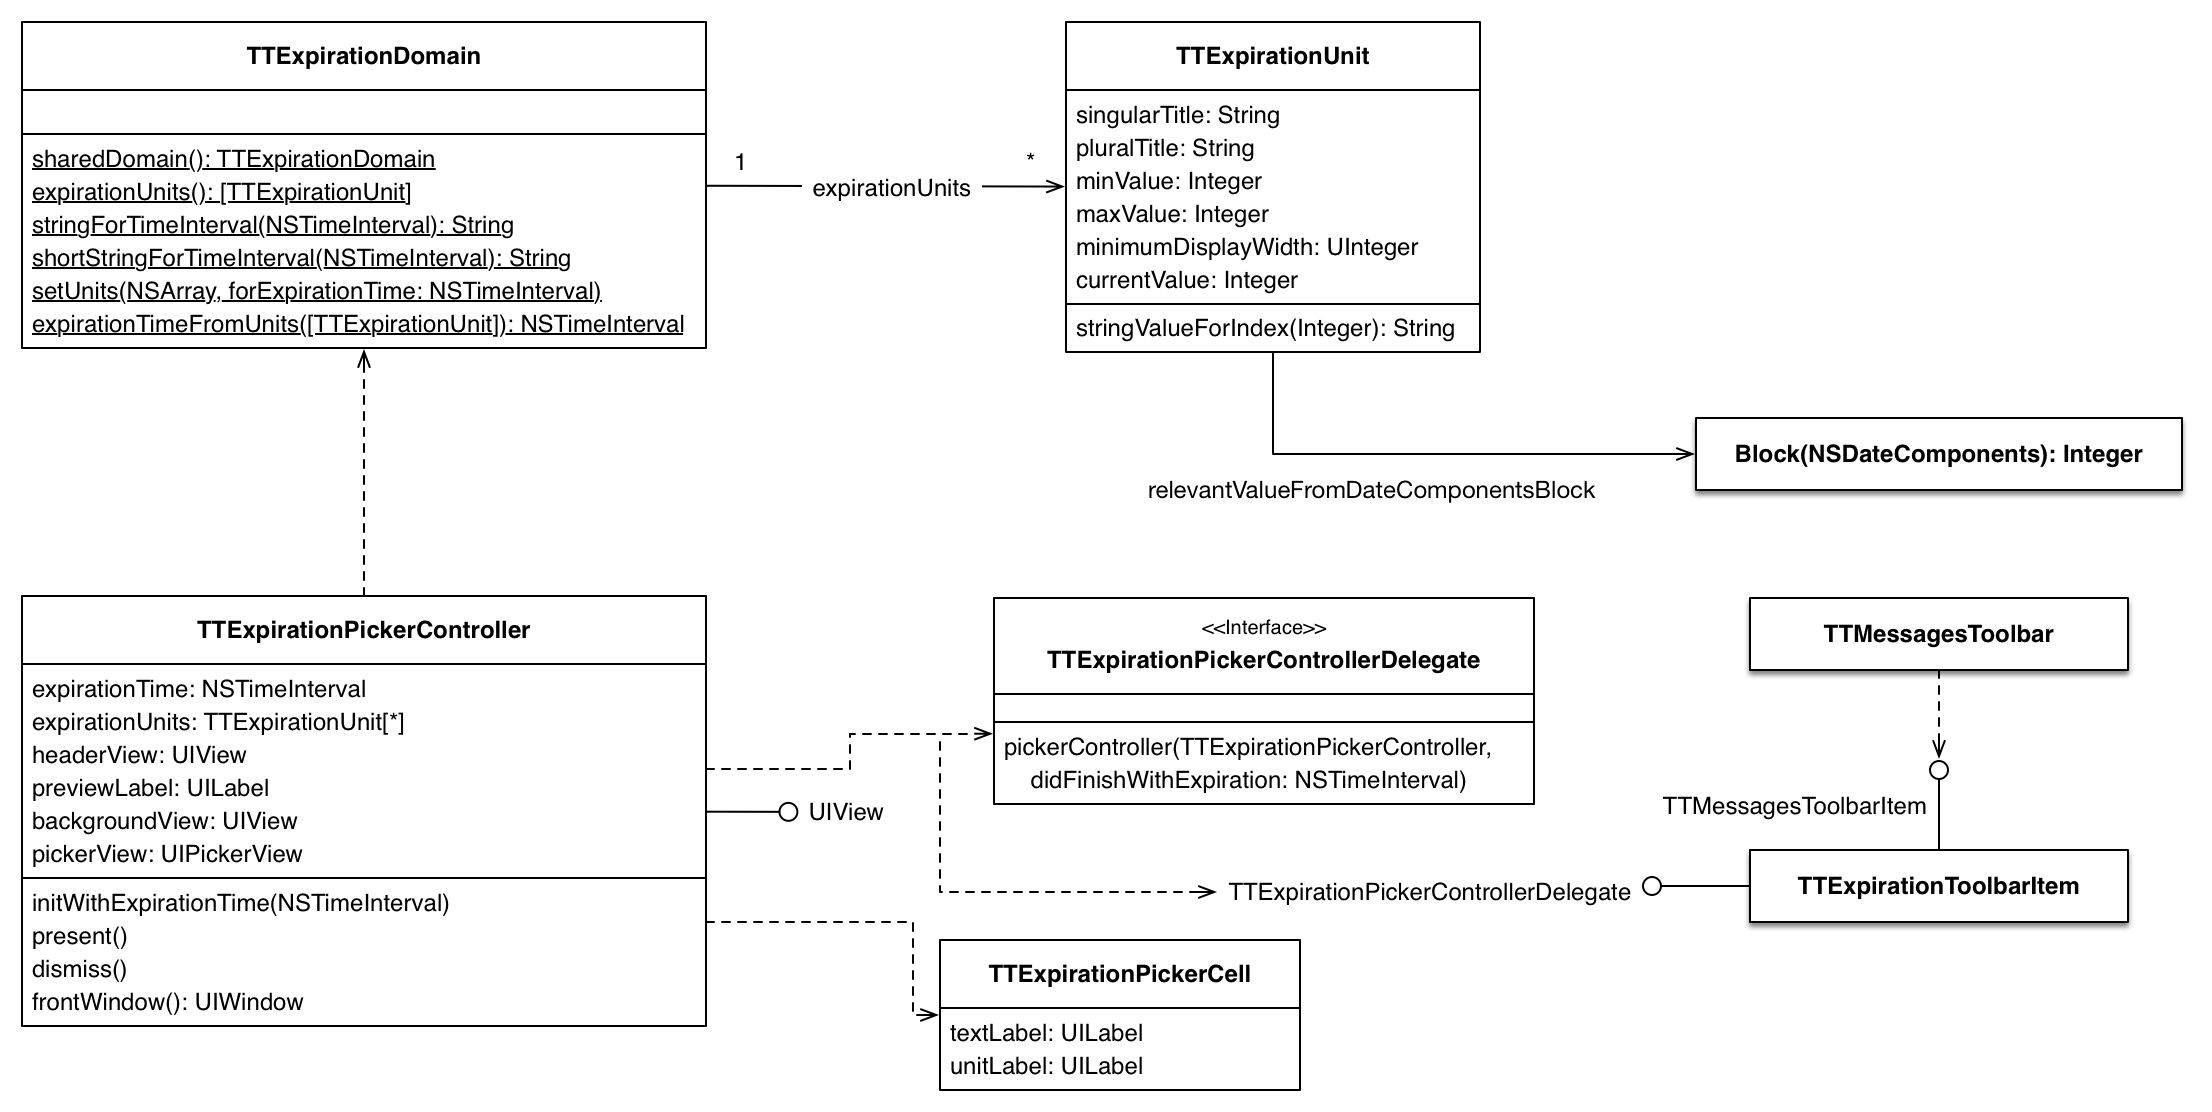
\includegraphics[width=\textwidth]{expirationpicker_class}
    \caption{Expiration Picker Class Diagram}
    \label{fig:expirationpicker_classdiagram}
\end{figure}

\begin{figure}[H]
    \centering
    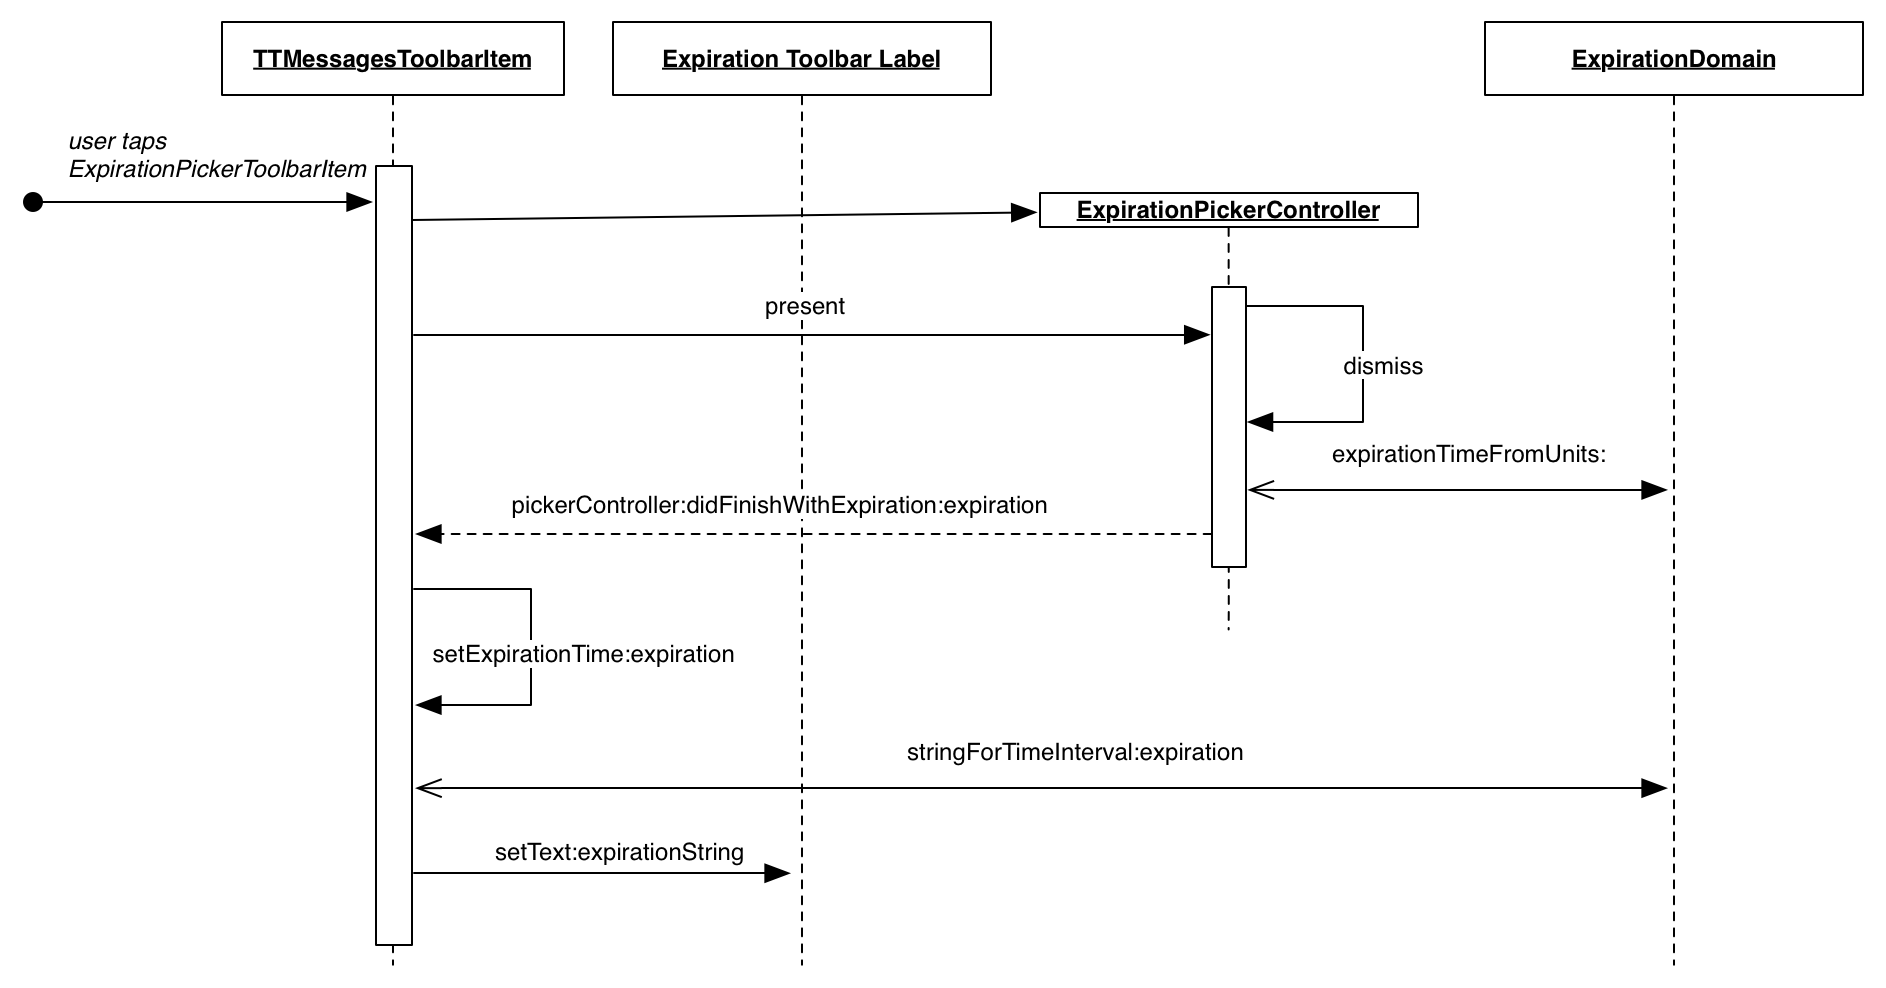
\includegraphics[width=\textwidth]{expirationpicker_sequence}
    \caption{Expiration Picker Sequence Diagram}
    \label{fig:expirationpicker_sequence}
\end{figure}

\subsection{Sequence Diagrams}
\begin{figure}[H]
    \centering
    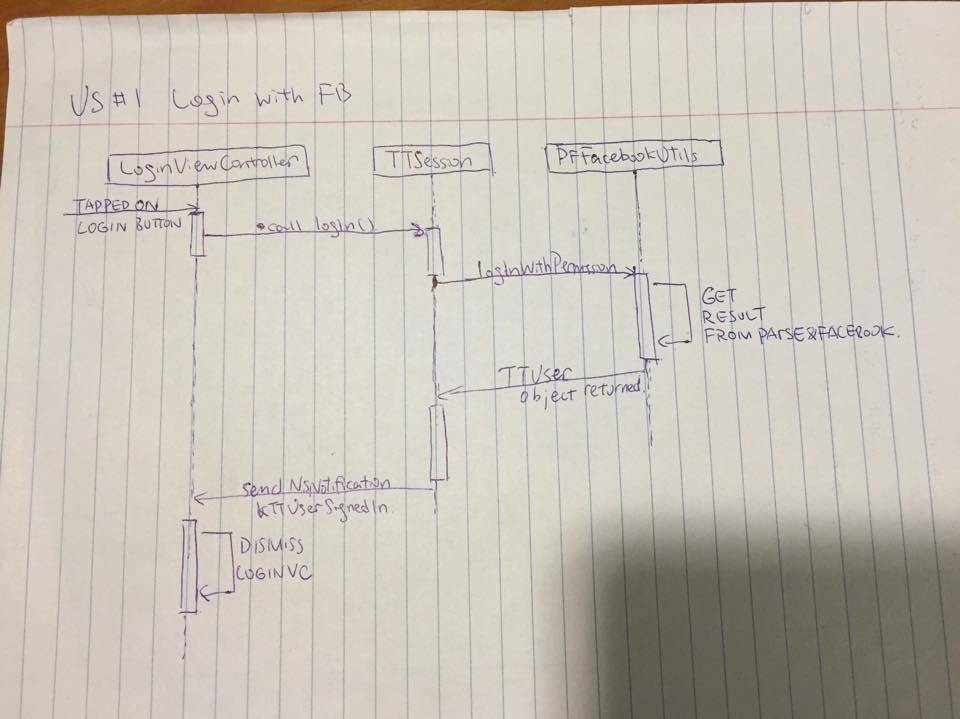
\includegraphics[width=0.8\textwidth]{us1_sequence}
    \caption{US1 Sequence Diagram}
    \label{fig:us1_sequence}
\end{figure}

\begin{figure}[H]
    \centering
    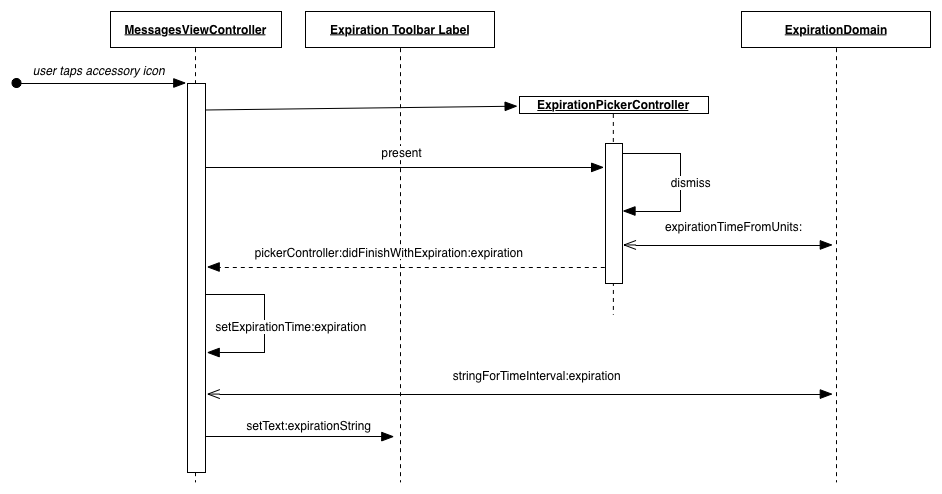
\includegraphics[width=0.8\textwidth]{us4_sequence}
    \caption{US4 Sequence Diagram}
    \label{fig:us4_sequence}
\end{figure}

\begin{figure}[H]
    \centering
    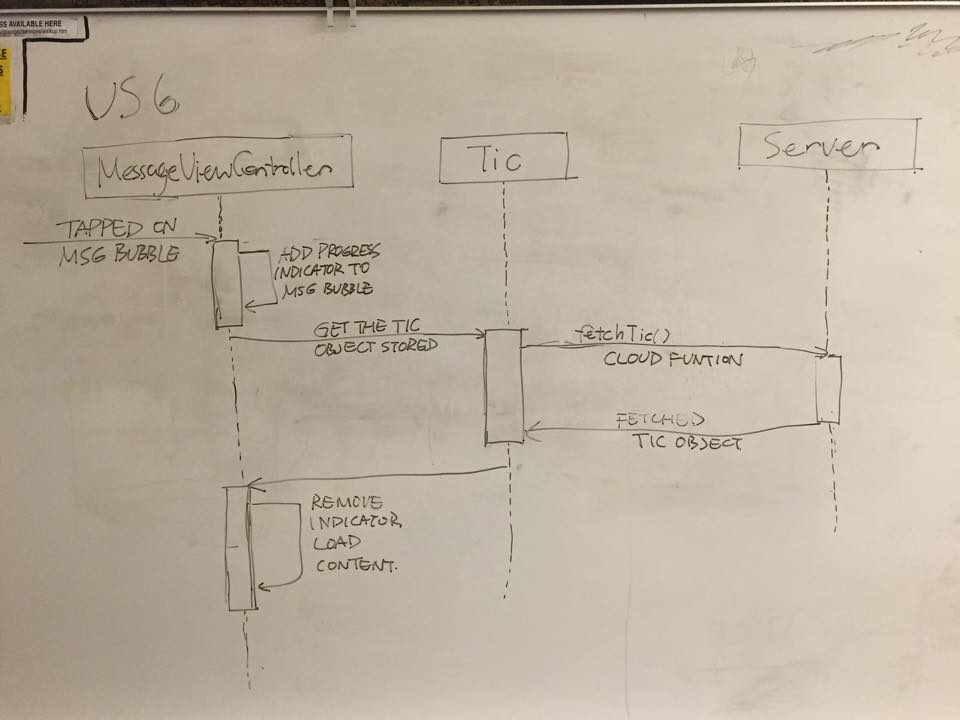
\includegraphics[width=0.8\textwidth]{us6_sequence}
    \caption{US6 Sequence Diagram}
    \label{fig:us6_sequence}
\end{figure}

\begin{figure}[H]
    \centering
    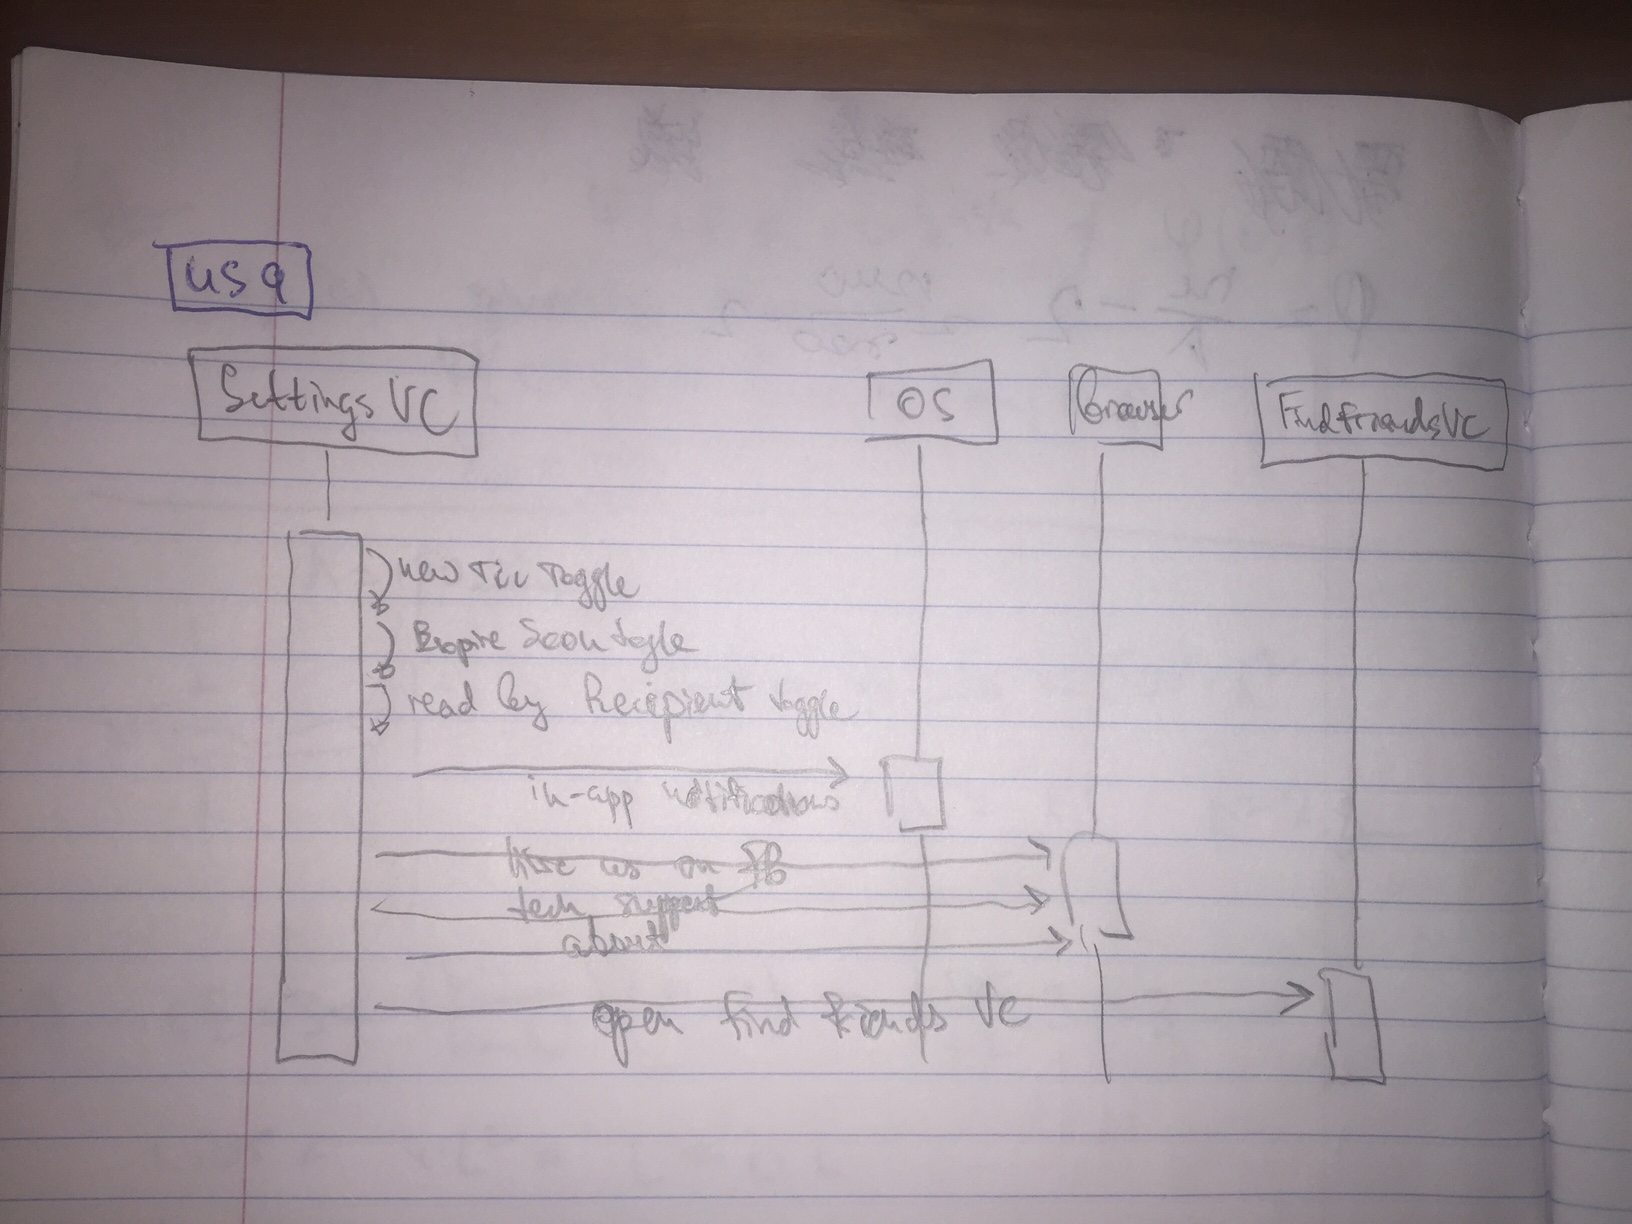
\includegraphics[width=0.8\textwidth]{us9_sequence}
    \caption{US9 Sequence Diagram}
    \label{fig:us9_sequence}
\end{figure}

\begin{figure}[H]
    \centering
    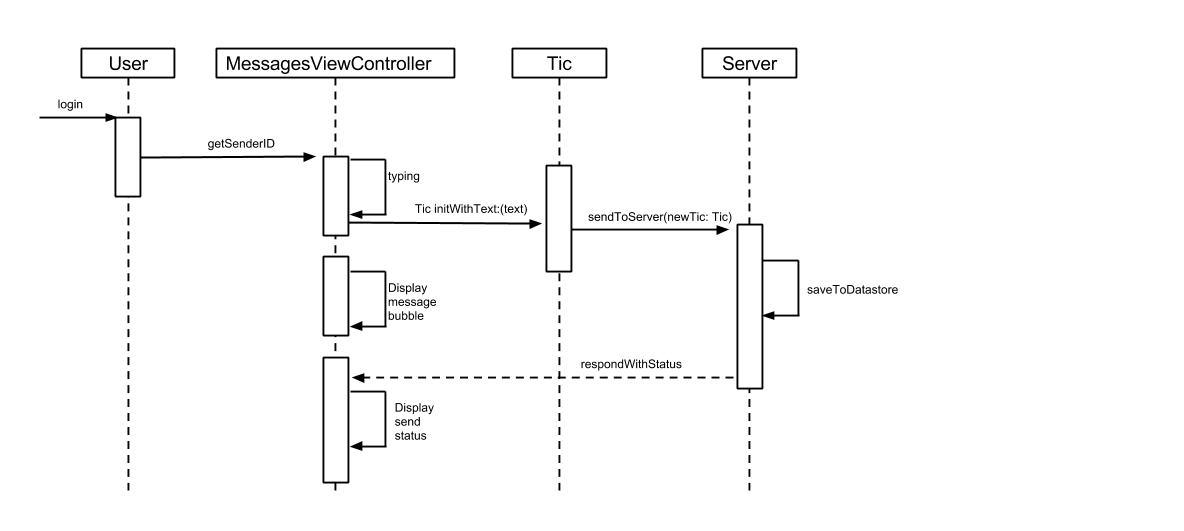
\includegraphics[width=0.8\textwidth]{us11_sequence}
    \caption{US11 Sequence Diagram}
    \label{fig:us11_sequence}
\end{figure}

\begin{figure}[H]
    \centering
    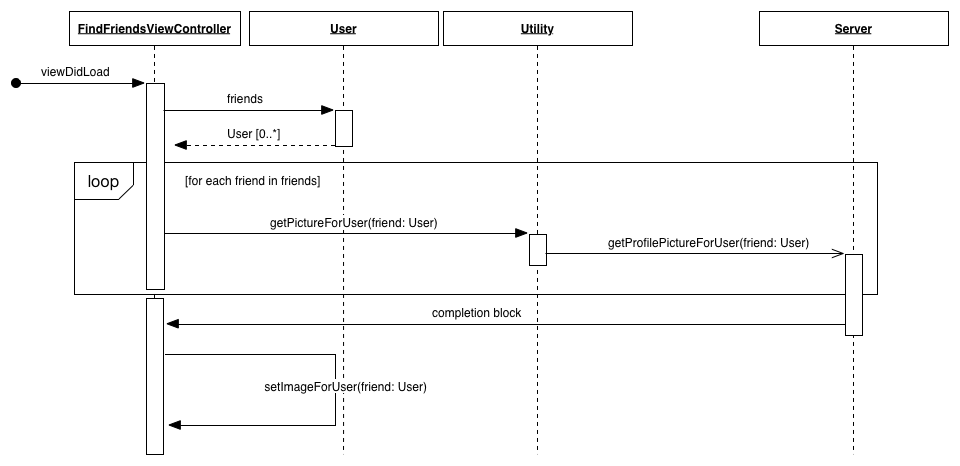
\includegraphics[width=0.8\textwidth]{us15_sequence}
    \caption{US15 Sequence Diagram}
    \label{fig:us15_sequence}
\end{figure}


% Future Plans
\clearpage
\section{Future Plans}
Future plans - (3 points)

Include personal reflections on the project and process by each team member. Describe what you learned.

% Terrence Katzenbaer
\begin{quote}
\lipsum[2]
\attrib{Terrence Katzenbaer}
\end{quote}

% Kevin Chen
\begin{quote}
\lipsum[2]
\attrib{Kevin Chen}
\end{quote}

% Chengkan Huang
\begin{quote}
\lipsum[2]
\attrib{Chengkan Huang}
\end{quote}

% Jack Arendt
\begin{quote}
\lipsum[2]
\attrib{Jack Arendt}
\end{quote}

% Georgy Petrukhov
\begin{quote}
\lipsum[2]
\attrib{Georgy Petukhov}
\end{quote}

\begin{table}[h]
	\centering
	\caption{Future Stories}
	 \renewcommand{\arraystretch}{1.2}
	\rowcolors{2}{white}{gray!20}
	\begin{tabular}{>{\centering\arraybackslash}m{2.5cm} | m{11.5cm} }
		\toprule
		Story Points & Description\\
		\midrule
		5 	& As a user, I want to send a voice message Tics to a TicText friend.\\
		3 	& As a user, I want to be able to set the app's color scheme in the in-app Settings\\
		5 	& As a user, I want to be able to set and sync a background image in a conversation (MsgVC) with my friend\\
		8 	& As a user, I want to be able to enter my phone number and have the app use my Address Book to automatically match us.\\
		3 	& As a user, I want to be able to check someone's profile from inside the conversation view.\\
		3 	& As a user, I want to be able to send a text with an invitation to join TicText to a person in my Address Book\\
		\bottomrule
	\end{tabular}
\end{table}


\end{document}
